\documentclass{article}

\usepackage[%
    left=0.5in,%
    right=0.5in,%
    top=0.5in,%
    bottom=0.5in,%
]{geometry}%
\usepackage{minitoc}
\usepackage{multicol}
\usepackage{graphicx}
\usepackage{fixltx2e}
\usepackage{listings}
\usepackage{color}
\usepackage{hyperref}
    \hypersetup{ colorlinks = true, linkcolor = blue }
\usepackage{blindtext}
\definecolor{lightgray}{gray}{0.9}
\graphicspath{ {./} }

\newcommand{\inlinecode}[2]{\colorbox{lightgray}{\lstinline
[language=#1]$#2$}}
\newcommand{\worddef}[1]{\hyperref[sec:reference]{\textit{#1}}}

\begin{document}

\tableofcontents

\newpage

\section{Quality assurance and standards}
\begin{itemize}
  \item Standards may be international, national, organizational or project based
  \item Product standards define characteristics that \textbf{all components should exhibit} e.g. a common programming style and how the software process should be enacted
\end{itemize}

\subsection{Importance of standards}
\begin{itemize}
  \item Encapsulation of best practice: \textbf{avoids repetition} of past mistakes
  \item Framework for quality assurance process: it involves \textbf{checking standard compliance}
  \item \textbf{Provide continuity}: new staff can understand the organisation by understand the standards applied
\end{itemize}

\subsection{The benefits of using standards}
\begin{itemize}
  \item The ability to \textbf{apply methodologies and procedures} of the highest professional level.
  \item Better \textbf{mutual understanding} and coordination amongst teams.
  \item \textbf{Greater cooperation} between the software developer and external participants in the project. Suppliers and customers, based on the adoption of standards \textbf{as part of the contract}.
\end{itemize}

\section{SQA classes}

\begin{center}
  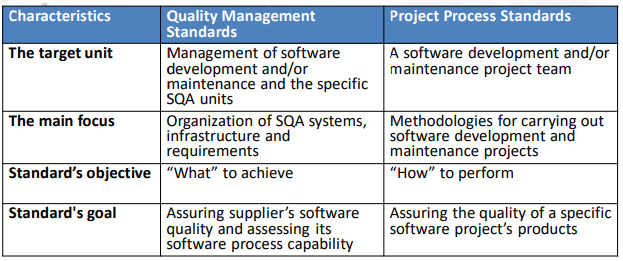
\includegraphics[scale=0.8]{sqa_classes.png}
\end{center}

\subsection{Certification standards}
\begin{itemize}
  \item Enable a software development organization to demonstrate \textbf{consistent ability} to assure acceptable quality of its software products or maintenance services. Certification is granted by an \textbf{external body}
  \item Serve as an agreed-upon basis for customer and \textbf{supplier evaluation} of the supplier’s quality management system. Accomplished by performance of a quality audit by the customer.
\end{itemize}

\subsection{Assessment standards}

\begin{itemize}
  \item Serve organizations as a \textbf{tool for self-assessment} of their ability to carry out software development projects.
  \item Serve for \textbf{improvement of development} and maintenance processes by application of the standard directions
  \item Help purchasing organizations \textbf{to determine the capabilities} of potential suppliers.
\end{itemize}

\section{ISO 9000}
\begin{flushleft}
International set of standards for quality management. Applicable to a range of organisations from manufacturing to service industries. \textbf{ISO 9001}:
\end{flushleft}
\begin{itemize}
  \item is the current standard to which organisations can be certified
  \item applicable to organisations which design, develop and maintain products
  \item is a generic model of the quality process that must be instantiated for each organisation
\end{itemize}

\subsection{ISO 9001 Certification}

\begin{flushleft}
Quality standards and procedures should be documented in an organisational quality manual. \textbf{External body} may certify that an organisation’s quality manual conforms to \textbf{ISO 9001} standards. Customers are, increasingly, demanding that suppliers are \textbf{ISO 9001} certified
\end{flushleft}

\subsection{ISO 9001 principles}

\begin{itemize}
  \item Customer focus
  \begin{itemize}
    \item Understand the needs of existing and future customers
    \item Align organizational objectives with customer needs and expectations
    \item Meet customer requirements
    \item Measure customer satisfaction
    \item Manage customer relationships
    \item Aim to exceed customer expectations
  \end{itemize}
  \item Leadership
  \begin{itemize}
    \item Establish a vision and direction for the organization
    \item Set challenging goals
    \item Model organizational values
    \item Establish trust
    \item Equip and empower employees
    \item Recognize employee contributions
  \end{itemize}
  \item Involvement of people
  \begin{itemize}
    \item Ensure that people’s abilities are used and valued
    \item Make people accountable
    \item Enable participation in continual improvement
    \item Evaluate individual performance
    \item Enable learning and knowledge sharing
    \item Enable open discussion of problems and constraints
    \end{itemize}  
  \item Process approach
  \begin{itemize}
    \item Manage activities as processes
    \item Measure the capability of activities
    \item Identify linkages between activities
    \item Prioritize improvement opportunities
    \item Deploy resources effectively
  \end{itemize}
  \item Continual improvement
  \begin{itemize}
    \item Improve organizational performance and capabilities
    \item Align improvement activities
    \item Empower people to make improvements
    \item Measure improvement consistently
    \item Celebrate improvements
  \end{itemize}  
  \item Factual approach to decision making
  \begin{itemize}
    \item Ensure the accessibility of accurate and reliable data
    \item Use appropriate methods to analyze data
    e Make decisions based on analysis
    \item Balance data analysis with practical experienc
  \end{itemize}  
  \item Mutually supportive supplier relationships
  \begin{itemize}
    \item Identify and select suppliers to manage costs, optimize resources, and create value
    \item Establish relationships considering both the short and long term
    \item Share expertise, resources, information, and plans with partners
    \item Collaborate on improvement and development activities
    \item Recognize supplier successes
  \end{itemize}
\end{itemize}

\section{Capability Maturity Model (CMM)}
\begin{flushleft}
The Capability Maturity Model (CMM) is a methodology used to develop and refine an organization's software development process.
\end{flushleft}
\begin{itemize}
  \item \worddef{Quantitative} management methods increases the organization's capability to control the quality and improve the productivity.
  \item Application of the five-level capability maturity model that enables to evaluate the achievements and determine the efforts needed to reach the next capability.
  \item Generic process areas that define the what, \textbf{not how} enables the model's applicability to a wide range of implementation organizations:
  \begin{itemize}
    \item Allows use of any life cycle model.
    \item Allows use of any design methodology, development tool and programming language.
    \item Does not specify any particular documentation standard.
  \end{itemize}
\end{itemize}

\subsection{Structure}

\begin{center}
  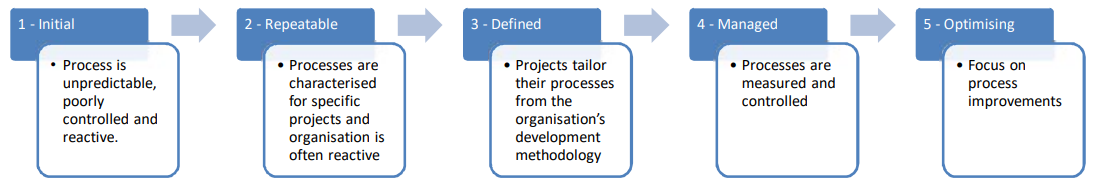
\includegraphics[scale=0.5]{cmm_structur.png}
\end{center}

\pagebreak

\subsection{Comparison of ISO 9000 vs CMM}

\begin{center}
  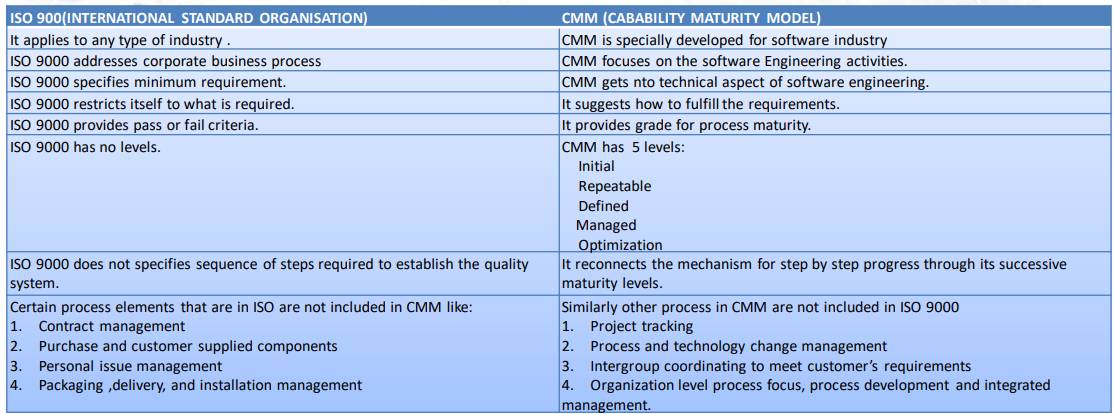
\includegraphics[scale=0.5]{cmm_vs_iso.png}
\end{center}

\section{Problems with standards}
\begin{itemize}
  \item Not seen as relevant and up-to-date by software engineers
  \item Involve too much bureaucratic form filling
  \item Unsupported by software tools so tedious manual work is involved to maintain standards
\end{itemize}

\subsection{Overcoming the Problems}

\begin{itemize}
  \item Involve practitioners in development: Engineers should understand the rationale underlying a standard
  \item Review standards and their usage regularly: Standards can quickly become outdated and this reduces their credibility amongst practitioners
  \item Detailed standards should have associated tool support: Excessive clerical work is the most significant complaint against standards
\end{itemize}

\section{Process and product quality}
\begin{quote}
The quality of a developed product is influenced by the \textbf{quality of the production process}
\end{quote}

\subsection{Process-based quality}

\begin{itemize}
  \item It's complex to link process to product because:
  \begin{itemize}
    \item The application of individual skills and experience is particularly
important in software development
    \item External factors such as the novelty of an application or the need for an
accelerated development schedule may impair product quality
  \end{itemize}
  \item Care must be taken not to impose \textbf{inappropriate process standards}
\end{itemize}

\subsection{Practical process quality}

\begin{itemize}
  \item \textbf{Define} process standards such as how reviews should be conducted,
configuration management, etc.
  \item \textbf{Monitor} the development process to ensure that standards are being followed
  \item \textbf{Report} on the process to project management and software procurer
\end{itemize}

\section{Quality planning}

\begin{itemize}
  \item A quality plan sets out the \textbf{desired product qualities} and how these are \textbf{assessed} and define the most \textbf{significant quality attributes}
  \item It should define the quality assessment process
  \item It should set out which organisational standards should be applied and, if necessary, define new standards.
\end{itemize}

\subsection{Structure}
\begin{quote}
Quality plans should be short, succinct documents – If they are too long, \textbf{no-one will read them}
\end{quote}

\begin{itemize}
  \item Product introduction
  \item Product plans
  \item Process descriptions
  \item Quality goals
  \item Risks and risk management
\end{itemize}

\section{Management and its role in software quality assurance}

\subsection{The quality assurance organisational framework (actors)}

\begin{flushleft}
Managers
\begin{itemize}
  \item Top management executives, especially the executive in charge of SQA
  \item Software development and maintenance department managers
  \item Software testing department managers
  \item Project managers and team leaders of development and maintenance projects
  \item Leaders of software testing teams
\end{itemize}
Testers
\begin{itemize}  
  \item Members of software testing teams
\end{itemize}
SQA professionals and interested practitioners
\begin{itemize}
  \item SQA trustees
  \item SQA committee members
  \item SQA forum members
  \item SQA unit team members
\end{itemize}
\end{flushleft}

\subsection{Top management’s overall responsibilities for software quality}

\begin{itemize}
  \item Assure the \textbf{quality} of the company’s software products and software \textbf{maintenance} services.
  \item Communicate the importance of product and service quality in addition to customer satisfaction to employees.
  \item Assure \textbf{full compliance} with customer requirements.
  \item Ensure that SQA objectives are established and accomplished.
  \item Initiate planning and \textbf{oversee implementation} of changes to adapt the SQA system to changes related to the organization's clientele, competition and technology.
  \item \textbf{Intervene directly} to resolve of crisis situations and minimize damages.
  \item \textbf{Ensure availability} of resources required by SQA systems.
\end{itemize}

\subsection{Software quality policy requirements}

\begin{flushleft}
Conformity to the organisation purpose and goals and commitment to:
\begin{itemize}
  \item General software quality assurance concepts
  \item The quality standards adopted by the organization
  \item Allocate adequate resources for software quality assurance
  \item Continuous improvement of the organizations quality and productivity
\end{itemize}
\end{flushleft}

\subsection{The responsibilities of the executive in charge of software quality}

\begin{itemize}
  \item Preparation of an annual SQA activities program and budget
  \item Preparation of SQA system development plans
  \item Overall control of implementation of the annual SQA regular activities program and planned SQA development projects
  \item Presentation and advocacy of SQA issues to executive management
\end{itemize}

\subsection{Typical items contained in management review reports}

\begin{flushleft}
\textit{Management review} is the name given to the periodic meeting convened to allow executives to obtain an overview of their organization’s software quality issues.
\begin{itemize}
  \item Periodic performance reports, including quality metrics
  \item Customer satisfaction feedback
  \item Follow up reports for SQA annual regular activity program and SQA development projects
  \item Summary of special quality events related to customers, suppliers, subcontractors, etc.
  \item Review of significant findings of internal and external quality audits as well as special surveys
  \item Identification of new software quality risks and unsolved pre-existing risks
  \item Recommendations for software quality management improvements.
\end{itemize}
\end{flushleft}

\subsection{The objectives of management reviews}

\begin{itemize}
  \item Assess achievement of quality objectives set for the organization’s SQM system
  \item Initiate updates and improvements of the SQM system and its objectives
  \item Outline directions for remedying major SQA deficiencies and software quality management problems.
  \item Allocate additional resources to the SQM system.
\end{itemize}

\subsection{Department management responsibilities for quality assurance}

\begin{flushleft}
The quality system-related responsibilities
\begin{itemize}
  \item Preparation of the department’s annual SQA activities program and budget, based on recommended SQA unit program.
  \item Preparation of the department’s SQA systems development plans, based on recommended SQA unit plan.
  \item Control of performance of the department’s annual SQA activities program and development projects
  \item Presentation of the department's SQA issues to the executive in charge of software quality
\end{itemize}
Project-related responsibilities
\begin{itemize}
  \item Control of compliance to QA procedures in the department's units
  \item Detailed follow up of contract review results and proposal approvals
  \item Review of unit performance of planned review activities; approval of project documents and project phase completion
  \item Follow up of software tests; approval of project’s software products
  \item Follow up of progress of software development project schedules and budget deviations. Advise and support project mangers in resolving difficulties
  \item Follow up of quality of maintenance services
  \item Detailed follow up of project risks and their solutions
  \item Follow up of project's compliance with customer requirements and customers satisfaction
  \item Approval of large software change orders and significant deviations from project specifications
\end{itemize}
\end{flushleft}

\subsection{Project management responsibilities for quality assurance}

\begin{flushleft}
Professional hands on tasks:
\begin{itemize}
  \item Preparation of project and quality plans and their updates.
  \item Participation in joint customer-supplier committee
  \item Close follow up of project team staffing, including recruitment, training and instruction.
\end{itemize}
Management tasks - The follow up issues:
\begin{itemize}
  \item Performance of review activities and the consequent corrections, including participating in some reviews.
  \item Software development and maintenance units’ performance with respect to development, integration and system test activities, corrections and regression tests and acceptance tests
  \item Software installation in customer sites and the running-in of the software system by the customer
  \item SQA training and instruction of project team members 
  \item Schedules and resources allocated to project activities. 
  \item Customer requests and satisfaction
  \item Evolving project development risks, application of solutions and control of results. 
\end{itemize}
\end{flushleft}

\section{Quality control}

\begin{flushleft}
Checking the software development process to ensure that procedures and standards are being followed. Two approaches to quality control: Quality reviews, Assessment via software metrics
\end{flushleft}

\subsection{Quality reviews}

\begin{itemize}
  \item The principal method of validating the quality of a process or of a product
  \item Group examines part or all of a process or system and its documentation to find potential problems
  \item There are different types of review with different objectives
  \begin{itemize}
    \item Inspections for defect removal (product)
    \item Reviews for progress assessment(product and process)
    \item Quality reviews (product and standards)
  \end{itemize}
\end{itemize}

\subsubsection{Purpose of Reviews}

\begin{itemize}
  \item Serve as a \textbf{filter} for the software process
  \item Uncover errors that can then be removed
  \item Purify the software analysis, design, coding, and testing activities
  \item Catch large classes of errors that escape the originator more than other practitioners
  \item Include the formal technical review (also called a walkthrough or inspection)
  \begin{itemize}
    \item Acts as the most effective SQA filter
    \item Conducted by software engineers for software engineers
    \item Effectively uncovers errors and improves software quality
    \item Has been shown to be up to 75\% effective in uncovering design flaws (which constitute 50-65\% of all errors in software)
  \end{itemize}
  \item Require the software engineers to expend time and effort, and the organization to cover the costs
\end{itemize}

\section{Formal Technical Review (FTR)}

\begin{itemize}
  \item \textbf{Objectives:}
  \begin{itemize}
    \item Uncover errors in function, logic, or implementation for any representation of the software
    \item Verify that the software under review meets its requirements
    \item Ensure that the software has been represented according to predefined standards
    \item Achieve software that is developed in a uniform manner
    \item Make projects more manageable
  \end{itemize}
  \item Serves as a \textbf{training ground} for junior software engineers to observe different approaches to software analysis, design, and construction 
  \item \textbf{Promotes backup and continuity} because a number of people become familiar with other parts of the software
  \item May sometimes be a sample-driven review
  \begin{itemize}
    \item Project managers must quantify those work products that are the primary targets for formal technical reviews
    \item The sample of products that are reviewed must be representative of the products as a whole
  \end{itemize}
\end{itemize}

\subsection{The FTR meeting}

\begin{itemize}
  \item Has the following constraints: From 3-5 people should be involved, advance preparation (i.e., reading) should occur for each participant \textbf{but should require no more than two hours} a piece and involve only a small subset of components, the duration of the meeting should be less than two hours
  \item Focuses on a specific work product (a software requirements specification, a detailed design, a source code listing)
\end{itemize}

\subsection{Before the FTR meeting}

\begin{itemize}
  \item The producer informs the project manager that a work product is complete and ready for review
  \item The project manager contacts a review leader, who evaluates the product for readiness, generates copies of product materials, and distributes them to the reviewers for advance preparation
  \item Each reviewer spends one to two hours reviewing the product and making notes before the actual review meeting
  \item The review leader establishes an agenda for the review meeting and schedules the time and location
\end{itemize}

\subsection{During the FTR meeting}

\begin{itemize}
  \item The meeting is attended by the review leader, all reviewers, and the producer
  \item One of the reviewers also serves as the recorder for all issues and decisions concerning the product
  \item After a brief introduction by the review leader, the producer proceeds to "walk through" the work product while reviewers ask questions and raise issues
  \item The recorder notes any valid problems or errors that are discovered; no time or effort is spent in this meeting to solve any of these problems or errors
\end{itemize}

\subsection{At the conclusion of the FTR meeting}

\begin{itemize}
  \item All attendees must decide whether to 
  \begin{itemize}
    \item \textbf{Accept} the product without further modification
    \item \textbf{Reject} the product due to severe errors (After these errors are corrected, another review will then occur)
    \item \textbf{Accept} the product provisionally (Minor errors need to be corrected but no additional review is required)
  \end{itemize}
  \item All attendees then complete a sign-off in which they indicate that they took part in the review and that they concur with the findings
\end{itemize}

\subsection{Following the FTR meeting}

\begin{itemize}
  \item The \textbf{recorder} produces a list of review issues that: \textbf{Identifies problem areas} within the product, Serves as an action item checklist \textbf{to guide the producer} in making corrections.
  \item The recorder includes the list in an FTR summary report: This one to two-page report describes \textbf{what} was reviewed, \textbf{who} reviewed it, and \textbf{what} were the findings and conclusions
  \item The review leader \textbf{follows up} on the findings to ensure that the producer makes the requested corrections
\end{itemize}

\subsection{FTR Guidelines}

\begin{itemize}
  \item Review the product, \textbf{not the producer}
  \item Set an agenda and maintain it
  \item \textbf{Limit} debate and rebuttal; conduct in-depth discussions off-line
  \item \textbf{Enunciate problem areas}, but don't attempt to solve the problem noted
  \item \textbf{Take written notes}; utilize a wall board to capture comments
  \item Limit the number of participants and insist upon advance preparation
  \item \textbf{Develop a checklist} for each product in order to structure and focus the review
  \item Allocate resources and schedule time for FTRs
  \item Conduct meaningful training for all reviewers
  \item Review your earlier reviews to \textbf{improve the overall review process}
\end{itemize}

\section{Quality Metrics}

\begin{itemize}
  \item Software measurement is concerned with \textbf{deriving a numeric value} for an attribute of a software product or process
  \item A software metric is any type of \textbf{measurement} which relates to a software system, process or related documentation
  \item This allows for \textbf{objective comparisons} between techniques and processes. There are few standards and no systematic use
\end{itemize}

\subsection{Quality attributes and software metrics}
\begin{itemize}
  \item \textbf{Maintainability}: the effort needed to make specified modifications. 
  \item \textbf{Reliability}: the capability of software to maintain its level of performance under stated conditions for a stated period of time. 
  \item \textbf{Portability}:  the ability of software to be transferred from one environment.
  \item \textbf{Usability}: the effort needed for use, and on the individual assessment of such use, by a stated or implied set of users.
\end{itemize}

\subsection{Important software metric assumptions}

\begin{itemize}
  \item A software property \textbf{can be measured}
  \item A relationship exists between what we can measure and a quality attribute
  \item This relationship has been formalized and validated
\end{itemize}

\subsection{The measurement process}

\begin{itemize}
  \item A software measurement process \textbf{may be part of} a quality control process
  \item Data collected during this process \textbf{should be maintained} as an organisational resource
  \item Once a measurement database has been established, \textbf{comparisons} across projects become possible
\end{itemize}

\subsection{Product metrics}

\begin{flushleft}
A quality metric should be a \textbf{predictor} of product quality. Classes of product metric:
\begin{itemize}
  \item Dynamic metrics
  \begin{itemize}
    \item Collected by a program in execution (response time, number of failures)
    \item Help assess efficiency, effectiveness, availability and reliability
  \end{itemize}
  \item Static metrics
  \begin{itemize}
    \item collected by measurements made of the system representations (lines of code)
    \item help assess complexity, understandability and maintainability
  \end{itemize}
\end{itemize}
\end{flushleft}

\section{Statistical software quality assurance}

\pagebreak
\section*{Reference section} \label{sec:reference}
\begin{description}
	\item[quantative] \hfill \\ relating to, measuring, or measured by the quantity of something rather than its quality.
\end{description}
\end{document}
